% Vorlesung vom 14.01.2016
\renewcommand{\ldate}{2016-01-14}
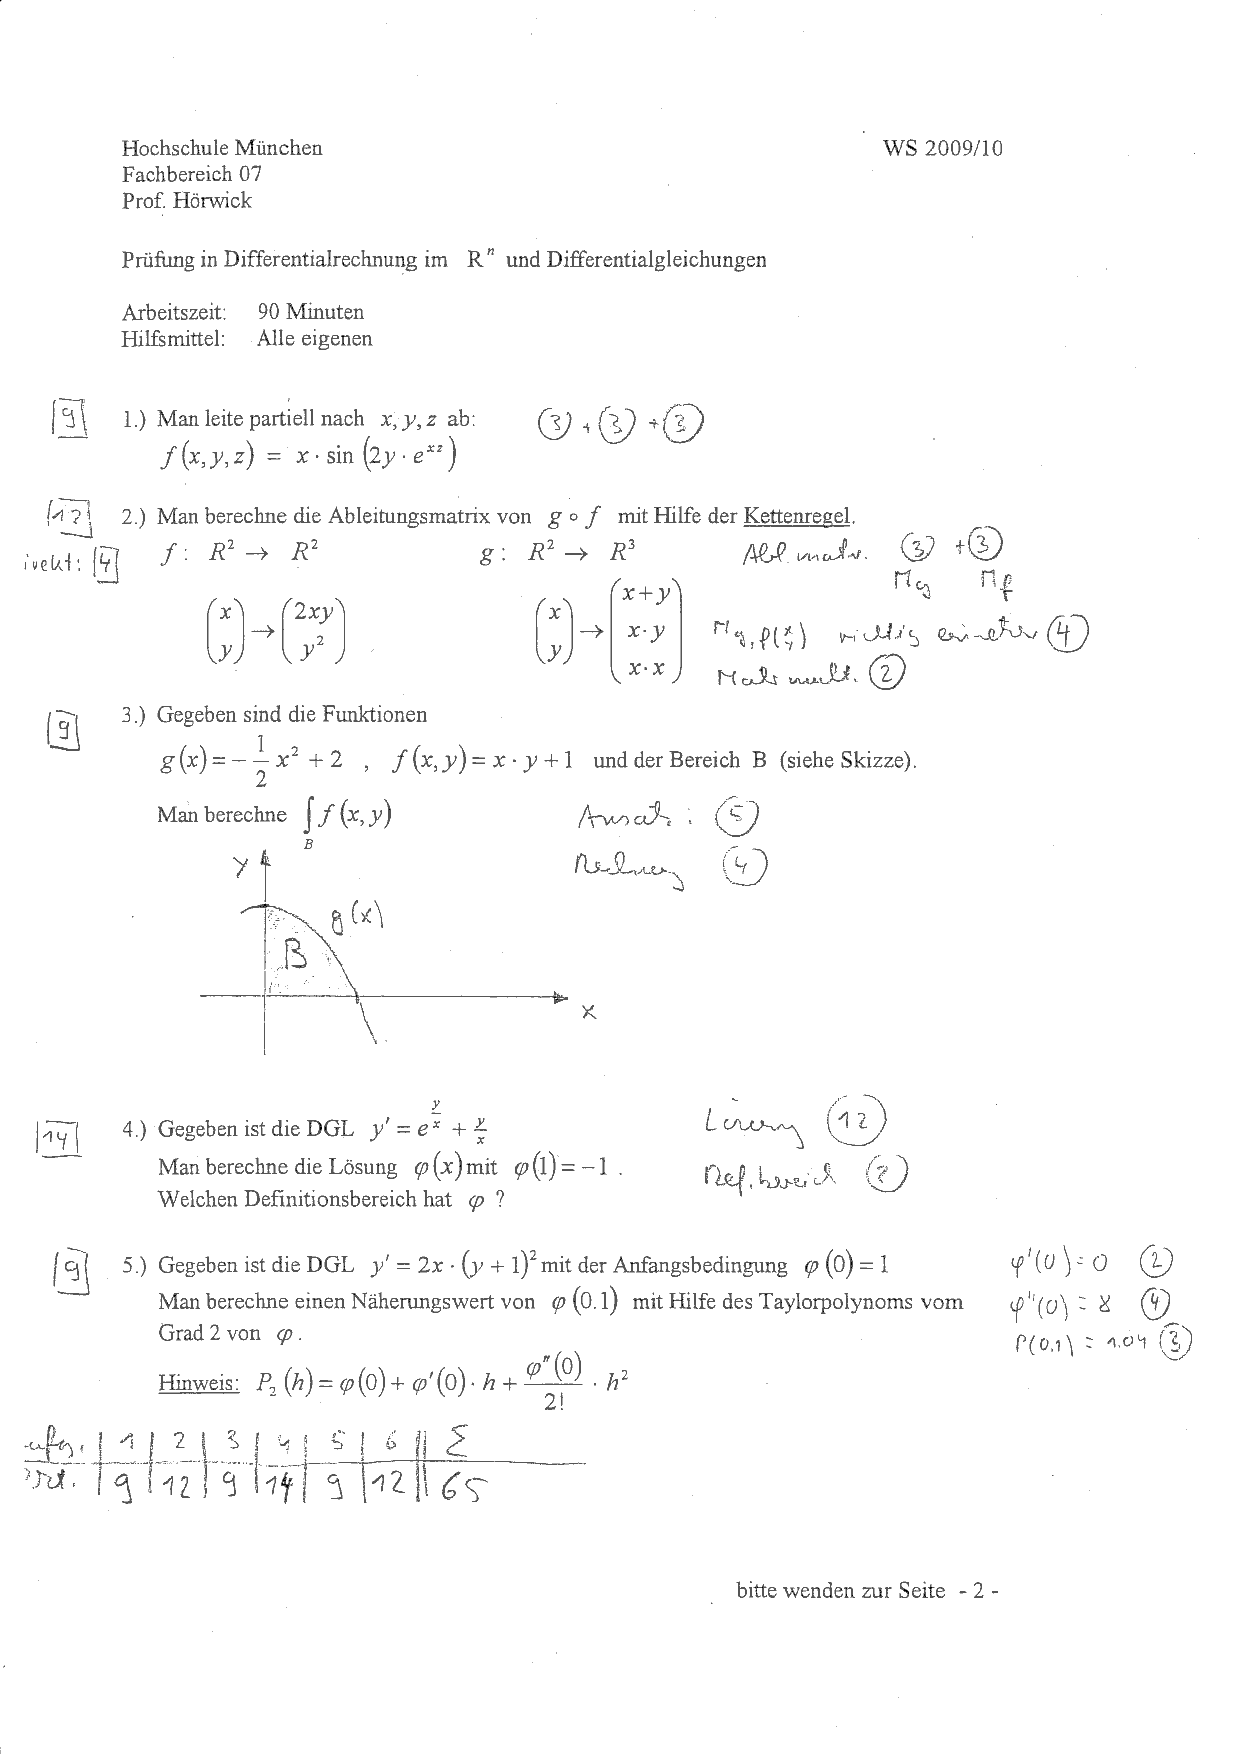
\includepdf[pages=-]{pruefungsangabe_diff_ws0910}

\section{Lösung für die Prüfung WS 2009/10}

\subsection{zu 1)}
$ f(x,y,z) = x \sin(2y e^{xz}) $ 

$ \frac{\df}{dx} = 1 \sin(2y\ e^{xz}) + x \cos(2y\ e^{xz}) 2y\ e^{xz} z $

$ \frac{\df}{dy} = x\cdot \cos(2y\ e^{xz}) \cdot 2e^{xz} $

$ \frac{\df}{dz} = x \cdot \cos(2y\ e^{xz}) \cdot 2y\ e^{xz} \cdot x $

\subsection{zu 2)}
$ f: \R^2 \rightarrow \R^2, \vektor{x\\y} \rightarrow \vektor{2xy\\y^2} $ und $ g: \R^2 \rightarrow \R^3, \vektor{x\\y} \rightarrow \vektor{x+y\\x\cdot y\\x\cdot x} $

$ (g\circ f)'(x) = g'(f(x)) \cdot f'(x) $

$ f'\vektor{x\\y} = \vektor{2y & 2x\\0 & 2y} $

$ g'\vektor{x\\y} = \vektor{1 & 1\\y & x\\2x & 0} $

$ (g\circ f)'\vektor{x\\y} = g' \rbr{f\vektor{x\\y}} \cdot f'\vektor{x\\y} 
= g'\vektor{2xy\\y^2} \cdot f'\vektor{x\\y}
= \vektor{1 & 1\\y^2 & 2xy\\4xy & 0} \cdot f'\vektor{2y & 2x\\0 & 2y}
= \vektor{2y & 2x + 2y\\2y^3 & 2xy^2 + 4xy^2\\8xy^2 & 8x^2y & 0}
$

Kontrolle: Berechne $ g\circ f$, dann ableiten. 

\subsection{zu 3)}
\profnote{Doppelintegral. Grenze des ersten Integrals ist die Nullstelle, hier: 2.}
$
\int_{B} f
= \int_{0}^{2} \sbr{ \int_{0}^{g(x)} f(x,y) dy} dx 
= \int_{0}^{2} \sbr{ \int_{0}^{g(x)} x\cdot y + 1 dy} dx
$

$
= \int_{0}^{2} \sbr{ x\cdot \frac{1}{2} y^2 + y}_{y=0}^{g(x)=y=-\frac{1}{2} x^2 + 2} dx  
= \int_{0}^{2} \sbr{\frac{1}{2} x \cdot \rbr{-\frac{1}{2} x^2 + 2}^2 + \rbr{-\frac{1}{2} x^2 + 2} } dx
= ...
= 4
$

\subsection{zu 4)}
$ y' = \frac{y}{e^x} + \frac{y}{x} $ mit $\varphi(1) = -1$ und der Substitution 
$ z = \frac{y}{x},  y=z\cdot x, y' = z' \cdot x + z \cdot 1 \Rightarrow z' \cdot x + z = e^z + z \Leftrightarrow z' = \frac{1}{x} \cdot e^z$ (Typ: getrennte Variable)\\

Lösung $\psi, \psi(1) = \frac{-1}{1}=-1$:

$ \int_{z_0}^{\psi(x)} \frac{1}{e^t} dt = \int_{x_0}^{x} \frac{1}{t} dt$ \profnote{Jetzt brauchen wir eine Stammfunktion}

$ \sbr{- e^{-t}}_{\psi(1) = -1}^{\psi(x)} = \sbr{\ln \abs{t}}_1^x $ mit $x>0$

$ (-e^{-\psi(x)}) - (-e^1) = \ln x - \ln 1 $ \profnote{einsetzen}

$ -e^{-\psi(x)} = \ln x - e $ \profnote{Nach $\psi(x)$ auflösen}

$ e^{-\psi(x)} = e - \ln x $

$-\psi(x) = \ln (e- \ln x)$

$\psi(x) = - \ln (e- \ln x)$\\

Lösung $\varphi(x) = x\cdot \psi(x) $

$\varphi(x) = - x \ln(e - \ln x)$\\

Definition von $\varphi(x) : x > 0$

$e - \ln x > 0 $

$e > \ln x$

\underline{$ e^e > x > 0 $}

\subsection{zu 5)}
Eine ähnliche Aufgabe haben wir bereits gerechnet. 

\subsection{zu 6)}
\renewcommand{\ldate}{2016-01-16}
\includegraphicsdeluxe{DrehPhi6.jpg}{Drehen}{Drehmatrix: $ \vektor{\cos \varphi & -\sin \varphi\\\sin \varphi & \cos \varphi} $}{fig:DrehPhi6}
Koordinaten von P im Hilfskoordinatensystem, dem u,v-System: 

$ \vektor{u\\v} = \underbrace{\vektor{\sin \varphi\\2 - \cos \varphi}}_{\textrm{um } \varphi \textrm{ drehen.}} $

$ \vektor{\cos \varphi & -\sin \varphi\\\sin \varphi & \cos \varphi} \vektor{\sin \varphi\\2-\cos \varphi} $
$=\vektor{\cos \varphi \sin \varphi - 2 \sin \varphi + \sin \varphi \cos \varphi\\\sin \varphi \sin \varphi + 2 \cos \varphi - \cos \varphi \cos \varphi } $

\section{Aufgaben und Wiederholungen}

\subsection{Zykloide}
Es wird auf Kapitel \ref{sec:die_zykloide} (Seite \pageref{sec:die_zykloide}) und Abb. \ref{fig:zykloid1} verwiesen. Weiterhin wird auf das s-t-Hilfskoordinatensystem und die dortigen Formeln für $ s(\varphi), x(\varphi) $ und $ y(\varphi) \Rightarrow f(\varphi) $ im selben Kapitel hingewiesen. 

\subsection{Linienintegral 1. Art}
Kurve im $\R^2, K(t)$

Funktion F: $\R^2 -> \R$

Die Skizze Abb. \ref{fig:LinInt1} auf Seite \pageref{fig:LinInt1} wird und das Integral $\int_{a}^{b} F(K(t)) \cdot \abs{K'(t)} dt$ wiederholt:

$ K(t) = \vektor{t\\t^2}, t=0 bis t = 2 $

$ F(x,y) = x\cdot y $

$ K'(t) = \vektor{1\\2t} $

$ \abs{K'(t)} = \sqrt{1 + 4 t^2} $

$ \int_{a}^{b} F(K(t)) \cdot \abs{K'(t)} dt 
= \int_0^2 F\vektor{t\\t^2} \cdot \sqrt{1 + 4t^2} dt
= \int_{0}^{2} t^3 \cdot \sqrt{1 + 4t^2} dt
= ?
$\profnote{Da, also bei ? hören wir auf. In der Prüfung käme im Fall der Fälle ein Integral vor, dessen Stammfunktion nicht zu schwer ist. Oder man muss es nur bis hier hin ausrechnen.}

\subsection{Linienintegral 2. Art (Arbeitsintegral)}
Auf Kapitel \ref{sec:linienintegral_arbeitsintegral} auf Seite \pageref{sec:linienintegral_arbeitsintegral} wird verwiesen. 

Formel für die Arbeit: $\int_{a}^{b} F(K(t)) \cdot K'(t) dt$ (Arbeitsintegral) 

\paragraph{Beispiel}
$ K(t) = \vektor{t\\2t}$ von $t=0$ bis $t=\pi$

Kraftfeld: $F\vektor{x\\y} = \vektor{\sin x\\\cos x}$

\profnote{Cave: Skalarprodukt!}
$ \int_{0}^{\pi} F\vektor{t\\2t} \cdot \vektor{1\\2} dt
=\int_{0}^{\pi} \vektor{\sin t\\\cos 2t} \cdot \vektor{1\\2} dt
=\int_{0}^{\pi} \sin t + 2\cos 2t dt 
= \sbr{-\cos t + \sin 2t}_{0}^{\pi}
= (-\cos \pi + \sin 2\pi) - (-\cos 0 + \sin 0)
= (1+0)-(-1+0)
= 2 
$ 
